\documentclass[article]{beamer}
\usetheme{Warsaw}
\setbeamertemplate{footline}[frame number]

\usefonttheme[]{serif}
\usepackage{amsmath, latexsym, color, graphicx, amssymb, bm, here}
\usepackage{epsf, epsfig, pifont,tikz,subfigure}
\usepackage{graphics, calrsfs}
\usepackage{times}
\usepackage{fancybox,calc}
\usepackage{palatino,mathpazo}
\usepackage{amsfonts}
\usepackage{sidecap}
\usepackage{listings}
\usepackage{hyperref}
\usepackage{algorithm, algorithmic}

\title{Graph Theory: Topological Sorting}
\author{David Jacobo \\ \href{mailto:jguillen@cimat.mx}{jguillen@cimat.mx}}
\date{\scriptsize{\today}}

\AtBeginSection[]
{
  \begin{frame}{Outline}
    \tableofcontents[currentsection]
  \end{frame}
}

\begin{document}

%%%%%%%%%%%%%%%%%%%%%%%%%%%%%%
\maketitle			
			
%%%%%%%%%%%%%%%%%%%%%%%%%%%%%%
\begin{frame}
\frametitle{Definition}
\begin{center}
\huge
	G = (V, E)
	
\vspace{8mm}	
	
%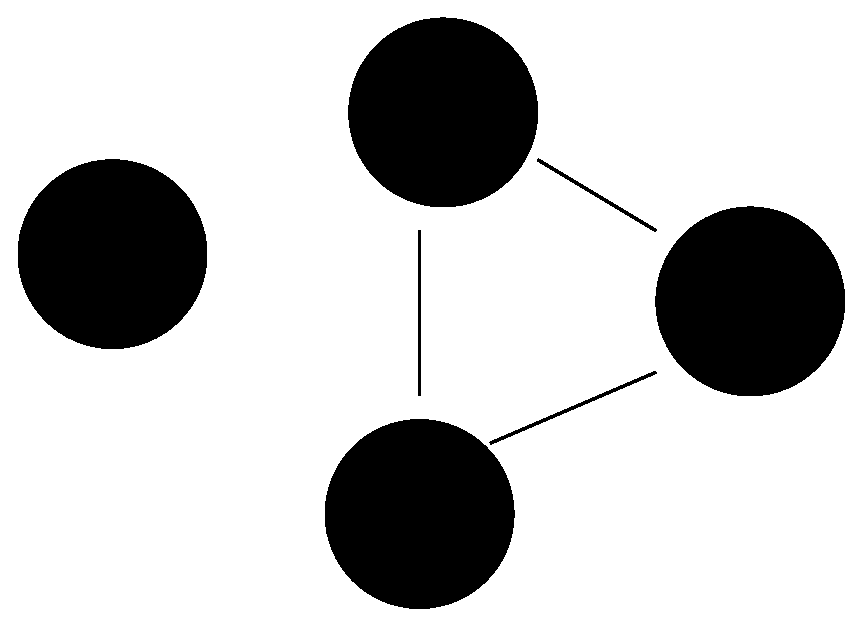
\includegraphics[scale=0.3]{./figures/graph.eps}
\end{center}
\end{frame}

\begin{frame}
\frametitle{Definition}
\begin{center}
Indegree: Basically tells us how many edges points to each of the vertices, $(u,v)$ augments v indegree in 1.
\end{center}
\end{frame}

%%%%%%%%%%%%%%%%%%%%%%%%%%%%%%

\section{Topological Sort}
\subsection{Intuition}
\begin{frame}
	\frametitle{Intuition}
	
	Given a directed-graph (aka \textbf{digraph}) in which the \textbf{vertices are tasks} and \textbf{edges represent dependencies between them}; tell if there is a permutation of the vertices which satisfies all the dependencies.

\end{frame}

%%%%%%%%%%%%%%%%%%%%%%%%%%%%%%%
\subsection{Algorithm}
\begin{frame}
	\frametitle{Algorithm}
	
		\begin{algorithm}[H]
		\begin{algorithmic}[1]
		\STATE $\forall$ $u$ $\in$ $V$, $u_{indegree}$ $\gets$ 0		
		\FOR{$u \in V$}
		\FOR{$v \in V$}
		\IF{$(u,v) \in G$}
		\STATE $v_{indegree} \gets v_{indegree} + 1$
		\ENDIF
		\ENDFOR
		\ENDFOR		
		
		\end{algorithmic}
		\caption{Compute indegree}
		\label{alg:seq}
		\end{algorithm}	
	
\end{frame}


\begin{frame}
	\frametitle{Algorithm}
	
		\begin{algorithm}[H]
		\begin{algorithmic}[1]			
		\FOR{$u$ $\in$ $V$ }
		\IF{$u_{indegree} == 0$}
		\STATE $output \gets output + u$
		\ENDIF
		\ENDFOR
		
		\end{algorithmic}
		\caption{Set initial vertices}
		\label{alg:seq}
		\end{algorithm}	
	
\end{frame}
%%%%%%%%%%%%%%%%%%%%%%%%%%%%%%%%%

\begin{frame}
	\frametitle{Algorithm}
	
		\begin{algorithm}[H]
		\begin{algorithmic}[1]
		\STATE Compute indegree
		\STATE Set initial vertices			
		\FOR{$u \in output$}
		\FOR{$v \in V$}
		\IF{$(u,v) \in G$}
		\STATE $v_{indegree} \gets v_{indegree} - 1$
		\IF{$v_{indegree} == 0$}
		\STATE $output \gets output + v$
		\ENDIF
		\ENDIF
		\ENDFOR
		\ENDFOR
		
		\end{algorithmic}
		\caption{Top-sort}
		\label{alg:seq}
		\end{algorithm}	
	
\end{frame}


\subsection{Tips and tricks}
\begin{frame}
	\frametitle{Keep in mind...}
	\begin{itemize}
		\item Remember the \textbf{indegree} concept.
		\item Generalize the algorithm as a way to sort tasks in a linear way.
		\item Never try to memorize code, but rather implement your own version and stick with it :)
		\item Customize (Pimp?) your code based on the problem.
	\end{itemize}
\end{frame}

%%%%%%%%%%%%%%%%%%%%%%%%%%%%%%
\begin{frame}[plain]
\frametitle{}
\begin{center}
\Huge{\color{blue}{Q \& A}} \\
\vspace{5mm}
%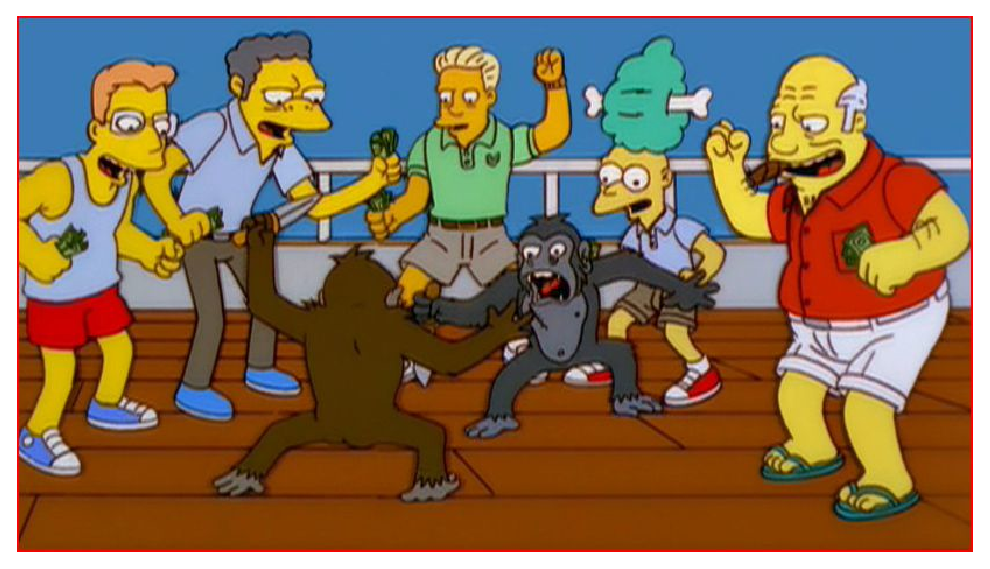
\includegraphics[scale=0.4]{./figures/monkey_fight.eps}
\end{center}
\end{frame}

%%%%%%%%%%%%%%%%%%%%%%%%%%%%%%%%
\begin{frame}[plain]
	\textbf{References}
	\begin{itemize}
		\item \href{https://sites.google.com/site/stevenhalim/}{Competitive Programming site}
		\item \href{https://github.com/davidjacobo/algorists/}{Algorists' repository}
	\end{itemize}
\end{frame}
\end{document}
